\documentclass[aspectratio=169,10pt]{beamer}

\usepackage[T1]{fontenc}
\usepackage[utf8]{inputenc}
\usepackage[english]{babel}
\usepackage{booktabs}
\usepackage{array}
\usepackage{graphicx}
\usepackage{tikz}
\usetikzlibrary{arrows.meta,positioning,fit,backgrounds,calc,shapes.misc}

% --------------------------------------------------
% Theme: metropolis in the CTU palette (same look as papers/2026-imeko-impulsive-sounds).
% --------------------------------------------------
\usetheme[progressbar=frametitle,numbering=fraction,block=fill,sectionpage=none]{metropolis}
\usepackage[sfdefault,lining]{FiraSans}
\usepackage{FiraMono}
\usepackage{newtxsf}
\usepackage{fontawesome5}

\definecolor{ctublue}{RGB}{0,101,189}
\definecolor{ctunavy}{RGB}{0,55,110}
\definecolor{accent}{RGB}{200,16,46}
\definecolor{ink}{RGB}{35,38,45}
\definecolor{paper}{RGB}{255,255,255}
\definecolor{panel}{RGB}{240,244,249}
\definecolor{okgreen}{RGB}{26,127,55}
% one colour per thesis, used as badges in the system diagram
\definecolor{tA}{RGB}{0,101,189}   % acoustic detection
\definecolor{tB}{RGB}{200,16,46}   % PDM acquisition
\definecolor{tC}{RGB}{26,127,55}   % localization survey
\definecolor{tD}{RGB}{214,120,0}   % web app
\definecolor{tE}{RGB}{110,60,160}  % IMU

\setbeamercolor{normal text}{fg=ink,bg=paper}
\setbeamercolor{structure}{fg=ctublue}
\setbeamercolor{alerted text}{fg=accent}
\setbeamercolor{example text}{fg=okgreen}
\setbeamercolor{frametitle}{fg=paper,bg=ctublue}
\setbeamercolor{progress bar}{fg=accent,bg=ctublue!30}
\setbeamercolor{block title}{fg=ctublue,bg=panel}
\setbeamercolor{block body}{bg=panel}
\setbeamercolor{block title alerted}{fg=paper,bg=accent}
\setbeamercolor{block body alerted}{bg=accent!8}
\setbeamercolor{block title example}{fg=paper,bg=okgreen}
\setbeamercolor{block body example}{bg=okgreen!8}
\setbeamercolor{footline}{fg=ink!55}
\setbeamercolor{page number in head/foot}{fg=ink!55}

\setbeamerfont{frametitle}{size=\large,series=\bfseries}
\setbeamerfont{block title}{series=\bfseries}
\setbeamerfont{footline}{size=\scriptsize}
\setbeamerfont{page number in head/foot}{size=\scriptsize}

\setbeamertemplate{navigation symbols}{}
\setbeamertemplate{itemize items}{\textcolor{ctublue}{\raisebox{0.15ex}{\rule{0.7ex}{0.7ex}}}}
\setbeamertemplate{enumerate items}[default]
\setbeamertemplate{frame footer}{Boomchecker \textperiodcentered\ Student kickoff 2026}
\makeatletter
\setlength{\metropolis@progressinheadfoot@linewidth}{1.2pt}
\setlength{\metropolis@frametitle@padding}{1.5ex}
\makeatother

% --------------------------------------------------
% Helpers
% --------------------------------------------------
\newcommand{\code}[1]{\texttt{#1}}
% Thesis badge: \badge{colour}{letter}
\newcommand{\badge}[2]{\tikz[baseline=(b.base)]\node[circle,fill=#1,draw=white,line width=0.8pt,text=white,inner sep=1.2pt,
  minimum size=3.6mm,font=\scriptsize\bfseries] (b) {#2};}

% Screenshot or a dashed TODO box when the file has not been added yet.
% \screenshot{file}{height}{what to capture}
\newcommand{\screenshot}[3]{%
  \IfFileExists{#1}%
    {\tikz\node[draw=ink!25,line width=0.6pt,inner sep=0pt]
      {\includegraphics[height=#2,width=\dimexpr\linewidth-1.2pt\relax,keepaspectratio]{#1}};}%
    {\tikz\node[draw=ink!40,dashed,line width=0.8pt,fill=panel,rounded corners=2pt,
      minimum height=#2,text width=0.92\linewidth,align=center,font=\small\color{ink!60}]
      {\faCamera\\[3pt]\textbf{TODO screenshot}\\[2pt]#3\\[2pt]\scriptsize\code{#1}};}}

% One slide per thesis: \thesis{colour}{letter}{title}{type / supervisor}{goal}{deliverables}{plugs in}
\newcommand{\thesis}[7]{%
  \begin{frame}{\badge{#1}{#2}\ #3}
    \textcolor{ink!65}{\small #4}\par\medskip
    \begin{columns}[T,onlytextwidth]
      \column{0.56\textwidth}
        \textbf{Goal}\par\smallskip
        {\small #5}\par\medskip
        \textbf{Where it plugs in}\par\smallskip
        {\small #7}
      \column{0.40\textwidth}
        \begin{block}{Key deliverables}\small #6\end{block}
    \end{columns}
  \end{frame}}

\tikzset{
  box/.style={draw=#1,fill=#1!8,rounded corners=2pt,line width=0.7pt,align=center,
    font=\small,inner sep=4pt},
  box/.default=ctublue,
  flow/.style={-{Latex[length=2mm]},line width=0.8pt,draw=ink!70},
  tag/.style={circle,fill=#1,text=white,inner sep=0pt,minimum size=3.8mm,font=\scriptsize\bfseries},
  % git graph
  c/.style={circle,draw=#1,fill=#1,minimum size=3mm,inner sep=0pt},
  c/.default=ctunavy,
  step/.style={box=#1,font=\scriptsize,inner sep=3pt},
  step/.default=ctublue,
  % kanban board
  col/.style={draw=ink!25,fill=panel,rounded corners=2pt,minimum width=24.5mm,minimum height=34mm,anchor=north},
  hd/.style={font=\scriptsize\bfseries,text=ctunavy,anchor=north},
  card/.style={draw=#1,fill=white,line width=0.6pt,rounded corners=1.5pt,minimum width=21mm,
    font=\scriptsize,align=left,text width=20mm,inner sep=2pt,anchor=north},
  card/.default=ink!40,
}

% --------------------------------------------------

\title{Drone Detection \& Localization}
\subtitle{Student kickoff: the project, the theses and how we work}
\author{Martin Maxa \and Kamil Herman \and Jakub Svatoš}
\institute{Czech Technical University in Prague\\Faculty of Electrical Engineering, Department of Measurement}
\date{Kickoff meeting, autumn 2026}

\begin{document}
\frenchspacing

% ==================================================
\begin{frame}[plain,noframenumbering]
  \begin{tikzpicture}[remember picture,overlay]
    \node[anchor=south west,inner sep=0pt] at (current page.south west)
      {
\includegraphics[width=\paperwidth,height=\paperheight]{figs/title-bg.png}};
    \node[anchor=north west,inner sep=0pt,xshift=9mm,yshift=-7mm] at (current page.north west)
      {
\includegraphics[height=12mm]{figs/electrical_engeneering_negativ.pdf}};
    \node[anchor=north west,text width=0.80\paperwidth,align=left,xshift=9mm,yshift=-26mm,
      text=paper] at (current page.north west) {%
        {\LARGE\bfseries\inserttitle\par}
        \vspace{2mm}
        {\large\insertsubtitle\par}
        \vspace{8mm}
        {\normalsize\insertauthor\par}
        \vspace{1.5mm}
        {\small\insertinstitute\par}
        \vspace{7mm}
        {\small\color{paper!80}\insertdate\par}
      };
  \end{tikzpicture}
\end{frame}

% ==================================================
\begin{frame}{Today}
  \begin{columns}[T,onlytextwidth]
    \column{0.55\textwidth}
      \begin{enumerate}
        \setlength{\itemsep}{6pt}
        \item \textbf{What we build}: drone detection as a system
        \item \textbf{The five theses}: who does what
        \item \textbf{How we develop}: repo, docs, devcontainers, git, AI
        \item \textbf{How we plan}: Kanban on GitHub Projects (live)
        \item \textbf{Next steps}
      \end{enumerate}
    \column{0.40\textwidth}
      \begin{block}{Joint meetings}
        \small
        Only three per semester:\\[2pt]
        \faFlag\ kickoff (today)\\
        \faAdjust\ mid-semester\\
        \faFlagCheckered\ end of semester\\[4pt]
        Everything else happens in individual consultations, whenever you need one.
      \end{block}
  \end{columns}
\end{frame}

% ==================================================
\section{What we build}

\begin{frame}{Why drone detection?}
  \begin{columns}[T,onlytextwidth]
    \column{0.52\textwidth}
      \begin{itemize}
        \setlength{\itemsep}{5pt}
        \item Small drones are cheap, everywhere, and hard to see.
        \item Many sensing principles exist: radar, RF, optical, thermal, \textbf{acoustic}.
        \item Acoustic units are \textbf{cheap, passive and low-power}, so we can build a network of them.
      \end{itemize}
      \vspace{6pt}
      \begin{alertblock}{Our goal}
        A \textbf{working end-to-end system}: sensor units in the field, a network, a backend
        and a map. We can then push detection as far as it goes.
      \end{alertblock}
    \column{0.44\textwidth}
      \centering
      \begin{tikzpicture}[font=\small]
        \node[box] (sense) {\faMicrophone\ \ \textbf{sense}\\[-1pt]\scriptsize mics, IMU, GPS};
        \node[box,below=4mm of sense] (detect) {\faWaveSquare\ \ \textbf{detect}\\[-1pt]\scriptsize on the node};
        \node[box,below=4mm of detect] (report) {\faBroadcastTower\ \ \textbf{report}\\[-1pt]\scriptsize LoRa to backend};
        \node[box=accent,below=4mm of report] (locate) {\faMapMarker*\ \ \textbf{locate \& show}\\[-1pt]\scriptsize fusion, map};
        \draw[flow] (sense)--(detect); \draw[flow] (detect)--(report); \draw[flow] (report)--(locate);
      \end{tikzpicture}
  \end{columns}
\end{frame}

% --------------------------------------------------
\begin{frame}{The system and where your thesis fits}
  \centering
  \begin{tikzpicture}[node distance=5mm and 9mm,font=\small]
    % sensor node
    \node[box,minimum width=27mm] (pdm) {PDM MEMS mics};
    \node[box,minimum width=27mm,below=3mm of pdm] (det) {detection /\\classification};
    \node[box,minimum width=27mm,below=3mm of det] (imu) {IMU + GPS\\\scriptsize orientation, position};
    \node[box,minimum width=27mm,below=3mm of imu] (lora) {LoRa BoomLink};
    \begin{scope}[on background layer]
      % "more nodes" shadows behind the main node
      \node[draw=ctunavy!25,fill=white,rounded corners=4pt,fit=(pdm)(lora),inner sep=6pt,xshift=8pt,yshift=-8pt] {};
      \node[draw=ctunavy!40,fill=white,rounded corners=4pt,fit=(pdm)(lora),inner sep=6pt,xshift=4pt,yshift=-4pt] {};
      \node[draw=ctunavy,line width=1pt,rounded corners=4pt,fill=panel,
        fit=(pdm)(lora),inner sep=6pt,label={[font=\small\bfseries,text=ctunavy]above:Sensor nodes (STM32H563)}] (node) {};
    \end{scope}
    \draw[flow] (pdm)--(det);

    % central side
    \node[box,right=12mm of lora] (gw) {gateway\\node};
    \node[box,right=of gw] (be) {backend\\\scriptsize ingest, storage};
    \node[box=accent,above=9mm of be] (loc) {localization\\\scriptsize multi-node fusion,\\[-2pt]\scriptsize TDOA / DoA};
    \node[box,right=of be] (web) {web map\\\scriptsize units, status, events};
    \draw[flow,dashed] (lora)--node[above,font=\scriptsize]{radio}(gw);
    \draw[flow] (gw)--(be);
    \draw[flow] (be.north)--(loc.south);
    \draw[flow] (be.east)--(web.west);

    % thesis badges
    \node[tag=tB] at (pdm.north east) {B};
    \node[tag=tA] at (det.north east) {A};
    \node[tag=tE] at (imu.north east) {E};
    \node[tag=tC] at (loc.north east) {C};
    \node[tag=tD] at (web.north east) {D};
    \node[tag=tD] at (be.north east) {D};
  \end{tikzpicture}

  \vspace{4pt}
  {\scriptsize
  \badge{tA}{A} detection \quad
  \badge{tB}{B} PDM acquisition \quad
  \badge{tC}{C} localization \quad
  \badge{tD}{D} web app \& telemetry \quad
  \badge{tE}{E} IMU orientation}
\end{frame}

% --------------------------------------------------
\begin{frame}{Honest limits: this is research}
  \begin{columns}[T,onlytextwidth]
    \column{0.48\textwidth}
      \begin{alertblock}{What we already know is hard}
        \small
        \begin{itemize}
          \item \textbf{Range}: sound attenuates fast and drones often fly high.
          \item \textbf{Noise}: wind, traffic, and the drone's own ego-noise.
          \item \textbf{Low power}: the node runs on a battery, so every mW counts.
        \end{itemize}
      \end{alertblock}
    \column{0.48\textwidth}
      \begin{exampleblock}{Where it can go next}
        \small
        \begin{itemize}
          \item \textbf{Microphone arrays}: direction of arrival, beamforming, more gain.
          \item \textbf{Sensor fusion}: acoustic + \textbf{RF detection}.
          \item Distributed networks of many cheap nodes.
        \end{itemize}
      \end{exampleblock}
  \end{columns}
  \vspace{10pt}
  \begin{center}
    \faRoute\ \ We \textbf{will} hit dead ends. That is fine as long as we measure them and write them down.\\[3pt]
    {\small\color{ink!65}Right now the priority is the \textbf{system itself}: make it work end to end first.}
  \end{center}
\end{frame}

% ==================================================
\section{The five theses}

\thesis{tA}{A}{Acoustic Drone Detection on the STM32 Platform}
  {\faUserGraduate\ \textbf{Jan Amos Vorel} \quad \faUserTie\ supervisor Martin Maxa}
  {Survey and compare features (spectral, MFCC / log-mel) and classifiers (classic ML, tiny NNs)
   for deciding \emph{drone / no drone} from short audio segments, with embedded deployment in mind.}
  {\begin{itemize}
     \item PC pipeline on real recordings
     \item accuracy, false alarms, behaviour under noise
     \item memory, compute and latency budget
     \item optional: feature extraction on STM32
     \item split: what runs on the node vs.\ centrally
   \end{itemize}}
  {The \textbf{detection} block on the sensor node. It builds on the existing MFCC + classifier
   code in \code{fw/common/boomdetect} and \code{fw/bom-stm32node/App/detect}.}

\thesis{tB}{B}{Firmware for Multi-Microphone PDM Acquisition on STM32H5}
  {\faUserGraduate\ \textbf{Ivan Dyryvolkov} \quad \faUserTie\ supervisor Martin Maxa}
  {Record 4--6 PDM MEMS microphones at once on the STM32H5 using SAI in PDM mode + DMA, and show
   that the channels are \textbf{time-synchronous}.}
  {\begin{itemize}
     \item clocks, SAI pins, DMA configuration
     \item buffer layout and de-interleaving to channels
     \item measured inter-channel delay
     \item data rate, CPU load, memory
     \item recommendations for DoA algorithms
   \end{itemize}}
  {The \textbf{microphone front-end} of the node and the enabler for microphone arrays. It starts from
   the single-mic SAI + GPDMA path in \code{fw/bom-stm32node} (\code{mic.c}, \code{pdm\_pcm.c}).}

\thesis{tC}{C}{Drone Localization Methods in UAV Detection Systems}
  {\faUserGraduate\ \textbf{Vojtěch Beneš} \quad \faUserTie\ supervisor Martin Maxa}
  {A systematic survey of how drones are localized (radar, RF, optical, thermal, \textbf{acoustic})
   with focus on direction of arrival, range estimation and distributed sensors.}
  {\begin{itemize}
     \item structured comparison of methods
     \item acoustic DoA, TDOA, multilateration
     \item distributed-sensor approaches
     \item promising directions for us
     \item simulation / public data / experiment
   \end{itemize}}
  {The \textbf{localization} block on the central side, and input for where we take the project next.
   Related code: \code{scripts/tdoa\_estimation}.}

\thesis{tD}{D}{Web App for Data Collection \& Map Visualization}
  {\faUserGraduate\ \textbf{Martin Voplakal} \quad \faUserTie\ supervisor Jakub Svatoš}
  {A web application for the network of detection units: the server receives, validates and stores
   telemetry, and a client map shows it in real time.}
  {\begin{itemize}
     \item survey of protocols and databases for telemetry
     \item backend architecture (battery, GPS, signal, events)
     \item choice of map API (Leaflet, MapLibre, Mapy.cz, \dots)
     \item responsive real-time UI
   \end{itemize}}
  {The \textbf{backend + web map} on the central side. A first version lives in \code{apps/api-backend} and \code{apps/device-web}, but the technology choice is yours.}

\thesis{tE}{E}{IMU Integration and Orientation Algorithms}
  {\faUserGraduate\ \textbf{Lumír Blažek} \quad \faUserTie\ supervisor Kamil Herman}
  {Know the node's \textbf{pitch, roll and yaw} so that acoustic measurements can be converted to
   global coordinates. This means accelerometer + gyro fusion with GPS drift correction.}
  {\begin{itemize}
     \item I2C/SPI + DMA driver (e.g.\ LSM6DS3)
     \item calibration and fusion algorithm
     \item tamper / fall detection
     \item SD-card logging, field tests
     \item low-power modes
   \end{itemize}}
  {The \textbf{IMU + GPS} block of the sensor node. Without orientation, a direction of arrival
   from the node cannot be placed on the map.}

\begin{frame}{Independent, but connected}
  \begin{columns}[c,onlytextwidth]
    \column{0.55\textwidth}
      \begin{itemize}
        \setlength{\itemsep}{6pt}
        \item The topics are designed so that \textbf{nobody waits for anybody}.
        \item Each thesis can be finished and defended on its own.
        \item But the outputs meet in one system, so \textbf{know what the others do}.
        \item Share what you learn: a working driver, a dataset or a dead end helps everyone.
      \end{itemize}
    \column{0.40\textwidth}
      \centering
      \begin{tikzpicture}[font=\small\bfseries]
        \node[tag=tA,minimum size=9mm,font=\normalsize\bfseries] (a) at (90:14mm) {A};
        \node[tag=tB,minimum size=9mm,font=\normalsize\bfseries] (b) at (162:14mm) {B};
        \node[tag=tC,minimum size=9mm,font=\normalsize\bfseries] (c) at (234:14mm) {C};
        \node[tag=tD,minimum size=9mm,font=\normalsize\bfseries] (d) at (306:14mm) {D};
        \node[tag=tE,minimum size=9mm,font=\normalsize\bfseries] (e) at (18:14mm) {E};
        \node[circle,draw=ctunavy,line width=1pt,minimum size=11mm,font=\scriptsize\bfseries,
          text=ctunavy,align=center] (s) at (0,0) {system};
        \foreach \n in {a,b,c,d,e} \draw[ink!40,line width=0.8pt] (\n)--(s);
      \end{tikzpicture}
  \end{columns}
\end{frame}

% ==================================================
\section{How we develop}

\begin{frame}[fragile]{One repository for everything}
  \begin{columns}[T,onlytextwidth]
    \column{0.55\textwidth}
      \small
      \begin{tabular}{@{}l>{\raggedright\arraybackslash}p{0.60\linewidth}@{}}
        \toprule
        \code{fw/}       & firmware (STM32 node, ESP32, shared libs) \\
        \code{apps/}     & backend, web, Discord bot \\
        \code{hw/}       & hardware (Altium) \\
        \code{scripts/}  & DSP experiments (TDOA, filters, \dots) \\
        \code{projects/} & self-contained student projects \\
        \code{papers/}   & publications and talks \\
        \code{docs/}     & documentation (MkDocs) \\
        \code{.devcontainer/} & dev environments \\
        \bottomrule
      \end{tabular}
    \column{0.40\textwidth}
      \begin{block}{Why a monorepo?}
        \small
        \begin{itemize}
          \item firmware, backend and docs change \textbf{together}
          \item one place to find code, docs and history
          \item the same rules and CI for everyone
        \end{itemize}
      \end{block}
      \vspace{4pt}
      {\small\faGithub\ \ \code{boomchecker-monorepo} on GitHub}
  \end{columns}
\end{frame}

% --------------------------------------------------
\begin{frame}{There is documentation. Read it!}
  \begin{columns}[T,onlytextwidth]
    \column{0.42\textwidth}
      \centering
      {\Large\faBook\ \ \textbf{docs.boomchecker.cz}}\par\bigskip
      \raggedright
      \textbf{Get Started}, top to bottom:\par\smallskip
      \small
      \begin{tikzpicture}[font=\small,node distance=1.2mm]
        \node[box,text width=52mm] (s1) {WSL2 \,\faAngleRight\, Docker \,\faAngleRight\, VS Code};
        \node[box,text width=52mm,below=of s1] (s2) {open the devcontainer};
        \node[box,text width=52mm,below=of s2] (s3) {share USB with usbipd};
        \node[box=okgreen,text width=52mm,below=of s3] (s4) {your first build};
        \node[box=ink,text width=52mm,below=of s4] (s5) {git basics \& contributing};
      \end{tikzpicture}\par
      \medskip
      {\scriptsize\color{ink!65}Docs are Markdown in \code{docs/}. When you add something others will use, document it
      in the same PR. Preview with \code{task docs:serve}.\par}
    \column{0.55\textwidth}
      % cropped to the left nav + page content (the file itself is the full window)
      \tikz\node[draw=ink!25,line width=0.6pt,inner sep=0pt]
        {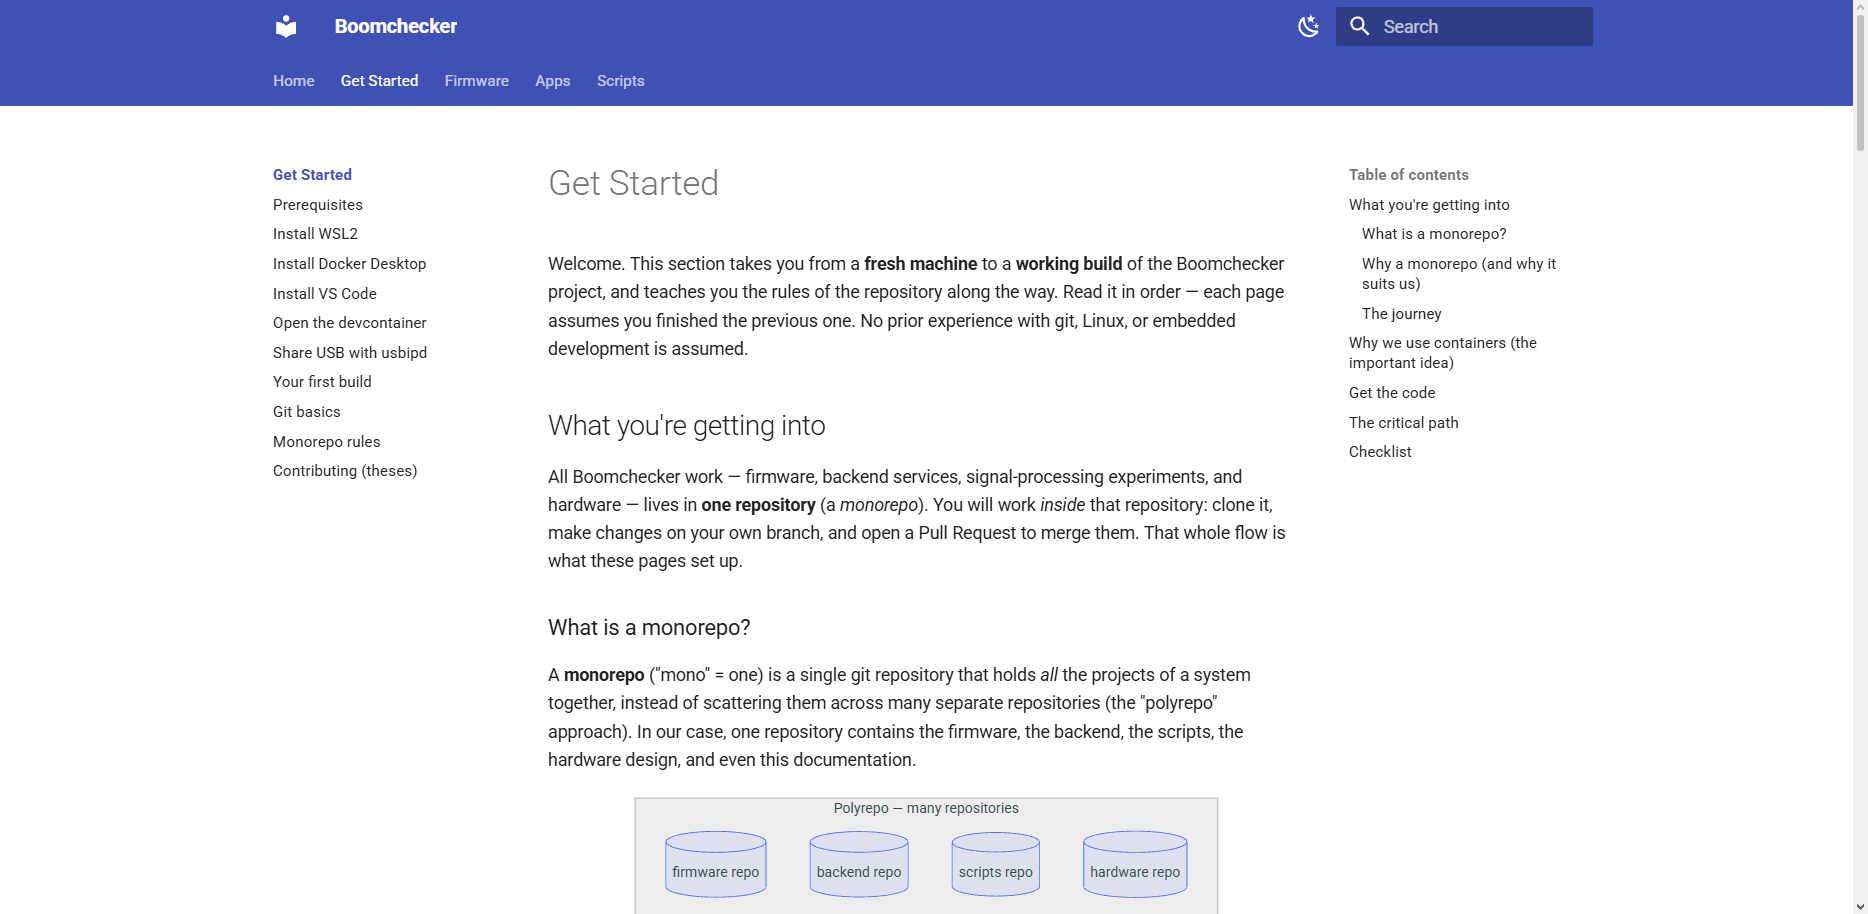
\includegraphics[width=\dimexpr\linewidth-1.2pt\relax,trim=240 170 520 0,clip]{figs/docs-screen.png}};
  \end{columns}
\end{frame}

% --------------------------------------------------
\begin{frame}{Devcontainers: the same toolchain for everyone}
  \begin{columns}[c,onlytextwidth]
    \column{0.58\textwidth}
      \centering
      \begin{tikzpicture}[font=\small,lay/.style={rounded corners=3pt,line width=0.7pt},
          ll/.style={font=\scriptsize\bfseries,anchor=north west,inner sep=2pt}]
        \draw[lay,draw=ink!70] (-1.4,-2.45) rectangle (5.0,2.35);
        \node[ll,text=ink] at (-1.4,2.35) {\faWindows\ Windows};
        \draw[lay,draw=ink!50,fill=panel] (-0.5,-0.95) rectangle (4.8,1.85);
        \node[ll,text=ink!70] at (-0.5,1.85) {\faLinux\ WSL2};
        \draw[lay,draw=ctublue,fill=ctublue!4] (-0.3,-0.75) rectangle (4.6,1.35);
        \node[ll,text=ctublue] at (-0.3,1.35) {\faDocker\ Docker};
        \node[box,minimum width=22mm] (fw) at (1.0,0.15) {\textbf{fw} container\\\scriptsize ESP-IDF, arm-gcc,\\[-2pt]\scriptsize OpenOCD, st-flash};
        \node[box,minimum width=22mm] (sw) at (3.4,0.15) {\textbf{sw} container\\\scriptsize Go, Python, Node,\\[-2pt]\scriptsize MkDocs};
        \node[box=ink] (vsc) at (0.2,-1.8) {\faCode\ VS Code};
        \node[box=accent] (usb) at (3.4,-1.8) {usbipd};
        \node[box=accent] (stl) at (3.4,-3.25) {\faUsb\ ST-Link / board};
        \draw[flow] (vsc.north) -- node[right,font=\scriptsize]{attaches} (vsc.north|-fw.south);
        \draw[flow,draw=accent] (stl.north) -- (usb.south);
        \draw[flow,draw=accent] (usb.north) -- ++(0,0.45) -| ([xshift=6mm]fw.south);
      \end{tikzpicture}
    \column{0.40\textwidth}
      \small
      \begin{itemize}
        \setlength{\itemsep}{4pt}
        \item \textbf{No manual toolchain install.} \emph{Reopen in Container} and you're done.
        \item \textbf{fw}: firmware for STM32 and ESP32, including flashing and debugging.
        \item \textbf{sw}: apps, scripts and docs.
        \item \textbf{usbipd} forwards the ST-Link / USB serial port from Windows into WSL and then the container.
        \item ``Works on my machine'' becomes ``works in the container''.
      \end{itemize}
  \end{columns}
\end{frame}

% --------------------------------------------------
\begin{frame}[fragile]{Taskfile: one entry point for commands}
  \begin{columns}[T,onlytextwidth]
    \column{0.50\textwidth}
      \small
      Instead of remembering long commands, we write them once in a \code{Taskfile.yml}:\par\medskip
      \scriptsize
\begin{verbatim}
$ cd fw/bom-stm32node
$ task -l        # what can I run here?
$ task build     # build the firmware
$ task flash     # flash over ST-Link
$ task monitor   # talk to the board
\end{verbatim}
    \column{0.45\textwidth}
      \begin{block}{Docker + Task = tools that save you time}
        \small
        \begin{itemize}
          \item the environment is defined by the devcontainer
          \item the commands are defined by Taskfiles
          \item you focus on your thesis, not on setup
        \end{itemize}
      \end{block}
      \vspace{4pt}
      {\scriptsize\color{ink!65}Add a task for anything you run more than twice.}
  \end{columns}
\end{frame}

% --------------------------------------------------
\begin{frame}{Where your work lives}
  \begin{columns}[T,onlytextwidth]
    \column{0.48\textwidth}
      \begin{exampleblock}{Working on our sensor unit?}
        \small
        Build on the \textbf{current firmware} in \code{fw/bom-stm32node} and add your part:
        a driver, a module, a task.\\[3pt]
        \textbf{Don't} start a fresh CubeMX project. We want one firmware that can do everything.
      \end{exampleblock}
    \column{0.48\textwidth}
      \begin{block}{Something standalone?}
        \small
        \code{projects/<year>-<name>-<topic>/}\\
        for your own experiments, reports and datasets.\\[4pt]
        \code{scripts/}: reusable DSP / analysis tools\\
        \code{apps/}: backend and web services
      \end{block}
  \end{columns}
  \vspace{8pt}
  \centering\small
  Not sure where something belongs? \textbf{Ask before you write 2000 lines.}
\end{frame}

% --------------------------------------------------
\begin{frame}[fragile]{Git basics we use every day}
  \begin{columns}[T,onlytextwidth]
    \column{0.54\textwidth}
      \textbf{Branch} from an up-to-date \code{main}:\par\scriptsize
\begin{verbatim}
git switch main && git pull
git switch -c yourname/short-description
\end{verbatim}
      \normalsize\textbf{Commit} small, logical steps:\par\scriptsize
\begin{verbatim}
git commit -m "feat(stmnode): add IMU driver"
git push -u origin yourname/short-description
\end{verbatim}
    \column{0.42\textwidth}
      \begin{block}{Conventional Commits}
        \small
        \code{\textcolor{ctublue}{type}(\textcolor{tD}{scope}): summary}\par\medskip
        \scriptsize
        \begin{tabular}{@{}>{\ttfamily\color{ctublue}}ll@{}}
          feat     & new feature \\
          fix      & bug fix \\
          docs     & documentation only \\
          refactor & code change, same behaviour \\
          test     & tests \\
          chore    & tooling, housekeeping \\
        \end{tabular}\par\medskip
        \small From our history:\par
        \scriptsize
        \code{feat(stmnode): drone SVM detector}\\
        \code{feat(boomlink): fleet discovery}\\
        \code{docs: add LoRa section}
      \end{block}
  \end{columns}
\end{frame}

% --------------------------------------------------
\begin{frame}{Protected \texttt{main} and pull requests}
  \centering
  \begin{tikzpicture}
    % main
    \draw[ctunavy,line width=2pt] (0,0) -- (13,0);
    \node[font=\small\bfseries,text=ctunavy,anchor=east] at (-0.2,0) {\faLock\ main};
    \foreach \x in {0.5,2,11.5,12.7} \node[c] at (\x,0) {};
    % feature branch
    \draw[ctublue,line width=1.6pt] (2,0) to[out=60,in=180] (3.4,1.4) -- (7.2,1.4);
    \foreach \x in {3.6,4.8,6.0,7.2} \node[c=ctublue] at (\x,1.4) {};
    \node[font=\scriptsize,text=ctublue,anchor=south] at (4.8,1.6) {\code{yourname/feature}: your commits};
    % PR steps
    \node[step] (pr) at (8.4,1.4) {\faCodeBranch\ PR};
    \node[step=okgreen] (ci) at (9.6,1.4) {\faCheck\ CI};
    \node[step=tD] (rv) at (10.85,1.4) {\faUserCheck\ review};
    \draw[ctublue,line width=1.6pt] (7.2,1.4) -- (pr.west);
    \draw[flow] (pr)--(ci); \draw[flow] (ci)--(rv);
    \draw[flow,ctunavy,line width=1.2pt] (rv.south) to[out=-90,in=150] (11.5,0.08);
    \node[font=\scriptsize,anchor=north] at (11.5,-0.15) {merge};
    % blocked push
    \draw[flow,accent,dashed] (5.4,-1.2) -- (5.4,-0.15);
    \node[font=\scriptsize,text=accent,anchor=north] at (5.4,-1.2) {\faBan\ direct push to \code{main} is rejected};
    \draw[flow,ink!50,dashed] (rv.north) to[out=90,in=90] node[above,font=\scriptsize,text=ink!60]{changes requested: push more commits} (6.0,1.55);
  \end{tikzpicture}

  \vspace{8pt}
  {\small \code{main} is protected: no direct pushes, every change lands through a reviewed PR.}
\end{frame}

% --------------------------------------------------
\begin{frame}{What it looks like on GitHub}
  \begin{columns}[T,onlytextwidth]
    \column{0.48\textwidth}
      \centering\textbf{Branch protection}\par\smallskip
      \screenshot{figs/branch-protection.png}{0.6\textheight}{branch protection rule for \code{main}}
    \column{0.48\textwidth}
      \centering\textbf{A pull request}\par\smallskip
      \screenshot{figs/pr-checks.png}{0.6\textheight}{PR with green checks + approval}
  \end{columns}
\end{frame}

% --------------------------------------------------
\begin{frame}{CI: the robot reviewer}
  \begin{columns}[T,onlytextwidth]
    \column{0.50\textwidth}
      Every PR is built and tested automatically by \textbf{GitHub Actions}:\par\medskip
      \small
      \begin{itemize}
        \setlength{\itemsep}{2pt}
        \item \code{test-bom-stm32node-build}: STM32 firmware
        \item \code{test-boomdetect-build}: detection library + tests
        \item \code{test-boomlink-protocol-build}: LoRa protocol
        \item \code{test-api-be-build}: Go backend
        \item \code{test-stm32node-cli}: Python host tool
        \item \code{docs-pages}: docs build (strict)
      \end{itemize}
    \column{0.45\textwidth}
      \begin{alertblock}{Red check = no merge}
        \small
        If CI fails, open the log, fix it, and push again. The PR updates by itself.
      \end{alertblock}
      \vspace{4pt}
      \begin{block}{Before you ask for review}
        \small
        \begin{itemize}
          \item it builds in the devcontainer
          \item the PR says \emph{what, why, how to test}
          \item no build output, secrets or unrelated files
        \end{itemize}
      \end{block}
  \end{columns}
\end{frame}

% --------------------------------------------------
\begin{frame}{AI tools: what CTU says}\relax
  {\small\textbf{Metodický pokyn č.\ 5/2023}: \emph{Rámcová pravidla používání umělé inteligence na ČVUT\dots}\par}
  {\scriptsize\color{ink!65}version V02, in force since 19 Feb 2024 \quad
    \faLink\ \href{https://www.cvut.cz/legislativa-tykajici-se-studia}{cvut.cz/legislativa-tykajici-se-studia}\par}
  \smallskip
  \begin{columns}[T,onlytextwidth]
    \column{0.48\textwidth}
      \begin{block}{General principles (Art.\ 1, 3)}
        \small
        \begin{itemize}
          \setlength{\itemsep}{2pt}
          \item CTU \textbf{supports} responsible, ethical use.
          \item Stay \textbf{independent}: you must reach the same results without AI.
          \item AI use must be \textbf{clearly declared and described}.
          \item \textbf{The author is responsible} for all AI errors
            (false claims, non-existent literature).
          \item No personal, sensitive or NDA data: the provider sees everything.
        \end{itemize}
      \end{block}
    \column{0.48\textwidth}
      \begin{exampleblock}{Programming (Art.\ 4.2): partially}
        \small
        \begin{itemize}
          \setlength{\itemsep}{2pt}
          \item Follow your supervisor's rules.
          \item AI saves time and can even propose a whole solution.
          \item \textbf{The student is the author of the code}: know exactly what the generated code does
            and be able to modify it.
          \item You must be able to write the same program \textbf{without} these tools.
        \end{itemize}
      \end{exampleblock}
  \end{columns}
\end{frame}

% --------------------------------------------------
\begin{frame}{AI in the thesis text (Art.\ 4.1)}
  \small
  \renewcommand{\arraystretch}{1.25}
  \newcommand{\aiyes}{\textcolor{okgreen}{\faCheck\ yes}}
  \newcommand{\aipart}{\textcolor{tD}{\faAdjust\ partially}}
  \newcommand{\aino}{\textcolor{accent}{\faTimes\ no}}
  \begin{tabular}{@{}l l >{\raggedright\arraybackslash\scriptsize}p{0.52\textwidth}@{}}
    \toprule
    \textbf{Activity} & & \textbf{Note} \\
    \midrule
    grammar check          & \aiyes  & no need to declare \\
    rewording, editing     & \aiyes  & be critical, it can change the meaning; list the AI tool among the software used \\
    finding authors, institutions & \aiyes & verify, or consult your supervisor \\
    literature search      & \aipart & inspiration only, never the only source; AI hallucinates, verify everything \\
    text structure         & \aipart & you are the author and responsible for it; list the AI tool \\
    machine translation    & \aipart & only from/to a language you speak yourself \\
    \textbf{theses, results} & \aino & must be your own; text you cannot explain means a disciplinary procedure \\
    \textbf{citations}     & \aino   & AI often invents sources; verify every single one \\
    \bottomrule
  \end{tabular}
\end{frame}

% --------------------------------------------------
\begin{frame}{AI tools in practice}
  \begin{columns}[T,onlytextwidth]
    \column{0.48\textwidth}
      \begin{exampleblock}{\faCheck\ \ Good use}
        \small
        \begin{itemize}
          \item explaining a compiler or runtime error
          \item boilerplate: config, parsers, test scaffolding
          \item refactoring or optimizing code you wrote
          \item explaining unfamiliar code line by line (HAL, libraries, our firmware)
          \item a second opinion on your design
        \end{itemize}
      \end{exampleblock}
    \column{0.48\textwidth}
      \begin{alertblock}{\faTimes\ \ Not OK}
        \small
        \begin{itemize}
          \item generating the whole assignment and submitting it
          \item submitting code you cannot explain
          \item AI-written results or invented citations
        \end{itemize}
      \end{alertblock}
      \vspace{4pt}
      {\small At the defense you may be asked to explain \textbf{any line}. Not knowing it can mean
      failing and a disciplinary procedure.}
  \end{columns}
\end{frame}

% --------------------------------------------------
\begin{frame}{Our stance: use it, but stay the engineer}
  \begin{columns}[c,onlytextwidth]
    \column{0.55\textwidth}
      \begin{itemize}
        \setlength{\itemsep}{6pt}
        \item What you should learn here: \textbf{reading and navigating real code}, i.e.\ firmware,
          drivers, DSP.
        \item You \textbf{may generate code}, but you must understand it and think it through.
        \item Review AI output like a PR from a colleague you don't fully trust.
        \item If a thesis were \emph{about} agentic development, the rules would differ.
          These theses are not.
      \end{itemize}
    \column{0.40\textwidth}
      \begin{block}{Available in the devcontainers}
        \small
        Claude Code and Codex come pre-configured, and \code{.claude/skills} holds a few shared skills.\\[4pt]
        Mention the AI tools you used in the thesis's list of software.
      \end{block}
  \end{columns}
\end{frame}

% ==================================================
\section{How we plan}

\begin{frame}{Agile in five minutes}
  \begin{columns}[T,onlytextwidth]
    \column{0.52\textwidth}
      \begin{itemize}
        \setlength{\itemsep}{6pt}
        \item \textbf{Iterate}: small steps, each one working and testable.
        \item \textbf{Make work visible}: everyone sees what's in progress and what's blocked.
        \item \textbf{Limit work in progress}: finish one thing before you start three new ones.
        \item \textbf{Adapt}: a dead end is a result. Record it and change the plan.
      \end{itemize}
    \column{0.44\textwidth}
      \centering
      \begin{tikzpicture}[font=\small]
        \foreach \a/\t in {90/plan,-30/build,210/{test \& learn}}
          \node[box,minimum width=19mm] (n\a) at (\a:14mm) {\t};
        \draw[flow] (n90) to[bend left=25] (n-30);
        \draw[flow] (n-30) to[bend left=25] (n210);
        \draw[flow] (n210) to[bend left=25] (n90);
      \end{tikzpicture}\par\medskip
      {\scriptsize\color{ink!65}No sprints, no ceremonies. Just a \textbf{Kanban board} and consultations when you need them.\par}
  \end{columns}
\end{frame}

% --------------------------------------------------
\begin{frame}{Kanban on GitHub Projects}
  \centering
  \begin{tikzpicture}
    \foreach \i/\n in {0/Backlog,1/Todo,2/In progress,3/In review,4/Done} {
      \node[col] (c\i) at (\i*26mm,0) {};
      \node[hd] at ([yshift=-1.5mm]c\i.north) {\n};
    }
    \node[card] at ([yshift=-6mm]c0.north) {survey map APIs};
    \node[card] at ([yshift=-14mm]c0.north) {SD-card logging};
    \node[card] at ([yshift=-22mm]c0.north) {try log-mel CNN};
    \node[card=tE] at ([yshift=-6mm]c1.north) {IMU calibration\\\color{ink!60}@Lumír};
    \node[card=tC] at ([yshift=-17mm]c1.north) {TDOA simulation\\\color{ink!60}@Vojtěch};
    \node[card=tB,line width=1pt] at ([yshift=-6mm]c2.north) {SAI 4-ch PDM + DMA\\\color{ink!60}@Ivan};
    \node[card=tA] at ([yshift=-6mm]c3.north) {MFCC on PC, baseline\\\color{ink!60}PR \#123};
    \node[card=okgreen] at ([yshift=-6mm]c4.north) {devcontainer works\\\color{ink!60}closed};
  \end{tikzpicture}

  \vspace{6pt}
  \begin{columns}[T,onlytextwidth]
    \column{0.55\textwidth}
      \small
      \begin{itemize}
        \setlength{\itemsep}{2pt}
        \item one piece of work = one \textbf{issue}, assigned to you
        \item \textbf{you manage your own issues}: create, split, move and close them as you work
        \item PR description with \code{Closes \#N} closes the issue on merge
      \end{itemize}
    \column{0.40\textwidth}
      \centering\small
      \faDesktop\ \ \textbf{Live demo}\\[-1pt]
      {\scriptsize\color{ink!65}create issue, then branch, PR, merge, card moves to Done\par}
  \end{columns}
\end{frame}

% --------------------------------------------------
\begin{frame}{Issues and milestones}
  \begin{columns}[T,onlytextwidth]
    \column{0.47\textwidth}
      \begin{block}{Example issue}
        \small
        \textbf{Channels from the 4 PDM mics are not aligned}\par\smallskip
        \scriptsize
        \textit{Problem}: after de-interleaving, a clap shows up with a different delay in
        each channel.\par\smallskip
        \textit{Possible approach} (optional): check the SAI slot order and the DMA half/full
        buffer handling, then measure with a common test signal.
      \end{block}
      \vspace{4pt}
      {\small An issue only needs to \textbf{describe the problem}. How to solve it is a hint at most.\par}
    \column{0.49\textwidth}
      \centering
      \begin{tikzpicture}[font=\scriptsize]
        \node[box=accent,font=\small] (m) at (4.2,0) {\faFlagCheckered\\[1pt]\textbf{milestone}\\[-1pt]\scriptsize agreed together};
        \node[circle,fill=ctunavy,inner sep=2pt] (st) at (0,0) {};
        \node[below=1pt of st,font=\scriptsize] {now};
        \draw[flow,draw=ctublue] (st) to[out=40,in=180] node[pos=0.5,above,sloped]{your issues} (m.west);
        \draw[flow,draw=ctublue!60,dashed] (st) to[out=-10,in=200] (m.west);
        \draw[flow,draw=ctublue!35,dashed] (st) to[out=-50,in=220] node[pos=0.55,below,sloped]{another path} (m.west);
      \end{tikzpicture}\par\medskip
      \raggedright\small
      \begin{itemize}
        \setlength{\itemsep}{3pt}
        \item \textbf{Milestones}: the goals we agree on together.
        \item \textbf{The path is yours}: which issues, in which order.
        \item \textbf{Consult it along the way} so you don't spend weeks in a dead end.
      \end{itemize}
  \end{columns}
\end{frame}

% ==================================================
\section{Next steps}

\begin{frame}{Next steps}
  \begin{columns}[T,onlytextwidth]
    \column{0.55\textwidth}
      \begin{enumerate}
        \setlength{\itemsep}{6pt}
        \item \textbf{GitHub access}: send your GitHub username to Martin (\code{maxamart@fel.cvut.cz}).
        \item Go through \textbf{Get Started} and have the devcontainer running before the first consultation.
        \item Make your \textbf{first PR}: e.g.\ fix something unclear in the docs.
        \item Agree on your \textbf{milestones} with your supervisor, then create your issues.
        \item Book a \textbf{consultation} with your supervisor.
      \end{enumerate}
    \column{0.40\textwidth}
      \begin{block}{Dates}
        \small
        \faCalendar*\ mid-semester meeting: \textbf{TBD}\\
        \faCalendar*\ final meeting: \textbf{TBD}
      \end{block}
      \vspace{4pt}
      \begin{block}{Contacts}
        \small
        \faDiscord\ project Discord\\
        \faEnvelope\ Martin Maxa, Kamil Herman, Jakub Svatoš
      \end{block}
  \end{columns}
\end{frame}

\begin{frame}[standout]
  Questions?\par\bigskip
  {\normalsize\mdseries docs.boomchecker.cz}
\end{frame}

\end{document}
